\documentclass[11pt,a4paper]{article}

% ==================== PACOTES ====================
\usepackage[utf8]{inputenc}
\usepackage[T1]{fontenc}
\usepackage[brazil]{babel}
\usepackage{geometry}
\geometry{top=2.0cm, bottom=2.2cm, left=2.0cm, right=2.0cm}
\usepackage{graphicx}
\usepackage{float}
\usepackage{hyperref}
\usepackage{enumitem}
\usepackage{booktabs}
\usepackage{array}
\usepackage{amssymb}
\usepackage{xcolor}
\usepackage{listings}
\usepackage{tcolorbox}
\tcbuselibrary{skins,breakable}

% ==================== CORES E ESTILOS ====================
\definecolor{imeblue}{RGB}{0, 51, 102}
\definecolor{alertred}{RGB}{180, 20, 20}
\definecolor{homegreen}{RGB}{20, 110, 50}
\definecolor{theorypurple}{RGB}{90, 40, 130}
\definecolor{codebg}{RGB}{245, 247, 250}

\hypersetup{
    colorlinks=true,
    linkcolor=imeblue,
    urlcolor=imeblue
}

\lstset{
    backgroundcolor=\color{codebg},
    basicstyle=\ttfamily\small,
    breaklines=true,
    frame=single,
    rulecolor=\color{gray!40},
    showstringspaces=false,
    commentstyle=\color{homegreen},
    keywordstyle=\color{imeblue}\bfseries,
    literate={á}{{\'a}}1 {à}{{\`a}}1 {ã}{{\~a}}1 {â}{{\^a}}1
             {é}{{\'e}}1 {ê}{{\^e}}1 {í}{{\'i}}1 {ó}{{\'o}}1
             {õ}{{\~o}}1 {ô}{{\^o}}1 {ú}{{\'u}}1 {ç}{{\c{c}}}1
             {Á}{{\'A}}1 {É}{{\'E}}1 {Í}{{\'I}}1 {Ó}{{\'O}}1
             {Ú}{{\'U}}1 {Ç}{{\c{C}}}1
}

% Caixas didáticas personalizadas
\newtcolorbox{alertbox}[1]{
    colback=alertred!5!white,
    colframe=alertred,
    fonttitle=\bfseries,
    title={#1},
    breakable
}

\newtcolorbox{theorybox}[1]{
    colback=theorypurple!5!white,
    colframe=theorypurple,
    fonttitle=\bfseries,
    title={#1},
    breakable
}

\newtcolorbox{homebox}[1]{
    colback=homegreen!5!white,
    colframe=homegreen,
    fonttitle=\bfseries,
    title={#1},
    breakable
}

\newtcolorbox{labbox}[1]{
    colback=imeblue!5!white,
    colframe=imeblue,
    fonttitle=\bfseries,
    title={#1},
    breakable
}

% ==================== INÍCIO DO DOCUMENTO ====================
\begin{document}

\begin{center}
    {\Large \textbf{INSTITUTO MILITAR DE ENGENHARIA (IME)}}\\[0.15cm]
    {\large Programação Aplicada à Engenharia Elétrica (SE/3 - Eletrônica)}\\[0.1cm]
    {\Large \textbf{Guia Didático Passo a Passo: Entregável 1}}\\[0.1cm]
    {\normalsize \textit{Subsistema IIO no Linux Embarcado, Modelagem POO em C++ e Doxygen}}\\[0.3cm]
    \begin{tabular}{lp{10.5cm}}
        \toprule
        \textbf{Prazo Oficial (Classroom):} & \textbf{Segunda-feira, 26/10/2026 às 23:59} (Valor: \textbf{2,0 pts} / 800 pts) \\
        \textbf{Kit de Desenvolvimento:} & STMicroelectronics \textbf{STM32MP157D-DK1} (Linux OpenSTLinux) \\
        \textbf{Sensor do Grupo (Nº 3):} & Módulo de Obstáculo Infravermelho Reflexivo Digital (\textbf{HW-201} / LM393) \\
        \textbf{Objetivo da Entrega 1:} & Classe em C++ para leitura do sensor documentada com Doxygen (via link do commit final no GitHub) \\
        \bottomrule
    \end{tabular}
\end{center}

\vspace{0.2cm}

% ====================================================================
\section{Cronograma Confirmado e Avaliação da Entrega 1}
% ====================================================================

Pelo novo edital atualizado em \textit{15 de outubro de 2026} e pelas tarefas publicadas no Google Classroom, as datas oficiais de todas as etapas estão confirmadas (\textbf{atenção especial:} as Entregas 4 e 5 vencem juntas no dia \textbf{16/11/2026}):

\begin{center}
\begin{tabular}{llcp{7.8cm}}
    \toprule
    \textbf{Etapa} & \textbf{Prazo (23:59)} & \textbf{Valor} & \textbf{Descrição Oficial no Classroom / Edital} \\
    \midrule
    \textbf{Entrega 0} & \textbf{19/10/2026} (Seg) & Obrig. & Foto da conexão física do sensor com o kit \textbf{desligado}. \\
    \textbf{Entrega 1} & \textbf{26/10/2026} (Seg) & 2,0 pts & Código-fonte em C++ da classe de leitura documentada com Doxygen. \\
    \textbf{Entrega 2} & \textbf{02/11/2026} (Seg) & 2,0 pts & Programa funcional no kit + instruções de compilação/execução no \texttt{README.md}. \\
    \textbf{Entrega 3} & \textbf{09/11/2026} (Seg) & 2,0 pts & Envio da leitura via UDP para o servidor + documentação do protocolo. \\
    \textbf{Entrega 4} & \textbf{16/11/2026} (Seg) & 2,0 pts & Interface gráfica no PC (tempo real, histórico 30--60s e log/CSV). \\
    \textbf{Entrega 5} & \textbf{16/11/2026} (Seg) & 2,0 pts & \textbf{Mesmo dia da Entrega 4!} Vídeo de demonstração, apresentação e documentação completa no \texttt{README.md}. \\
    \bottomrule
\end{tabular}
\end{center}

\begin{figure}[H]
    \centering
    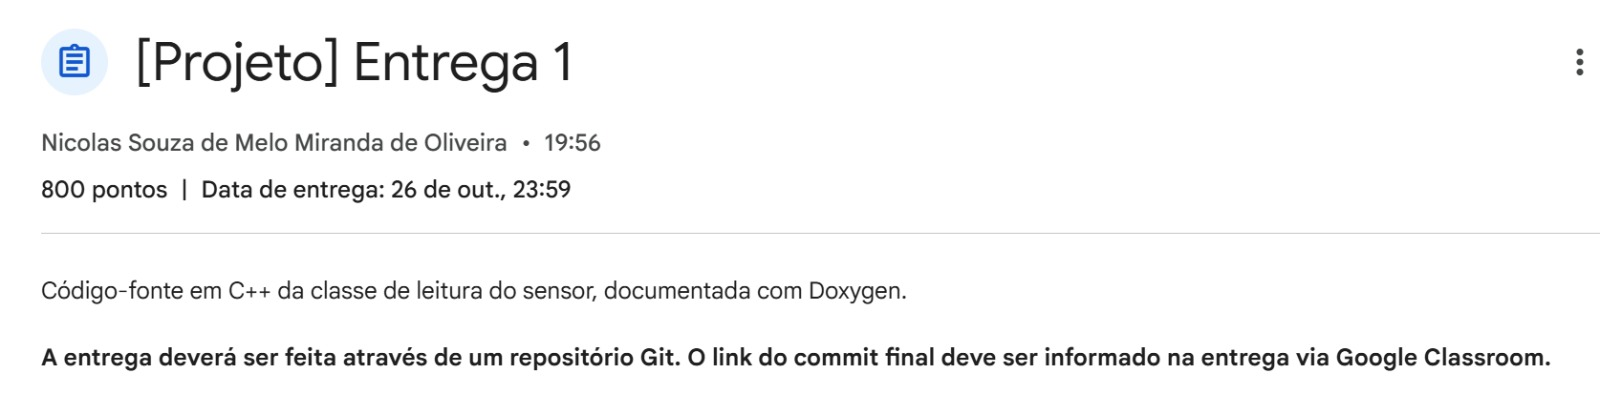
\includegraphics[width=0.78\textwidth]{latex_assets/classroom_entrega1.jpg}
    \caption{Tarefa oficial da Entrega 1 publicada no Google Classroom (26/10 às 23:59).}
\end{figure}

\begin{alertbox}{As 3 Regras de Ouro da Avaliação (Evite Penalizações)}
\begin{enumerate}[leftmargin=*]
    \item \textbf{Proibição Estrita de Variáveis Globais e Funções Soltas (Regra nº 2):} \\
    \textit{Por que o professor exige isso?} Porque na Entrega 5 (Simulação Integrada), o código dos 11 grupos da turma poderá ser integrado em um único sistema. Se dois grupos criarem uma variável global \texttt{int leitura;} ou uma função solta \texttt{lerSensor()}, haverá colisão de nomes (\textit{linker error}). Quando tudo está \textbf{encapsulado dentro da sua classe C++} (ex.: \texttt{class IrObstacleSensor}), cada sensor vive isolado dentro do seu próprio objeto!
    
    \item \textbf{Divisão Profissional de Arquivos (\texttt{.hpp} e \texttt{.cpp}):} \\
    Em C++, não colocamos tudo dentro de um único arquivo. Criamos um \textbf{arquivo de cabeçalho} (\texttt{include/IrObstacleSensor.hpp}) para declarar \textit{o que a classe tem e faz}, e um \textbf{arquivo de implementação} (\texttt{src/IrObstacleSensor.cpp}) para programar \textit{como cada método funciona}.
    
    \item \textbf{Documentação com Doxygen e Link do Commit Final:} \\
    A classe deve conter comentários especiais \texttt{/** ... */} acima da classe, dos atributos e dos métodos. A entrega no Google Classroom deve ser o \textbf{link direto do commit final} no GitHub do grupo.
\end{enumerate}
\end{alertbox}

% ====================================================================
\section{A Teoria: Como o Linux da Placa Lê um Pino Físico?}
% ====================================================================

Se você já programou em Arduino, deve lembrar da função \texttt{analogRead(A0)}. Mas na sua placa \textbf{STM32MP157D-DK1}, o código não roda ``direto no ferro'' (\textit{bare-metal}): ele roda dentro de um \textbf{Sistema Operacional Linux}.

\begin{theorybox}{No Linux, ``Tudo é um Arquivo'' (\textit{Everything is a File})}
No Linux, um programa comum de usuário é proibido de acessar registradores de memória física diretamente por questões de segurança. Em vez disso, o Kernel do Linux possui um driver chamado \textbf{IIO (\textit{Industrial I/O})} que conversa com o conversor Analógico-Digital (ADC) do chip STM32MP157D e cria ``arquivos virtuais'' na pasta:
\begin{center}
    \texttt{/sys/bus/iio/devices/iio:device0/}
\end{center}
Dentro dessa pasta existem arquivos chamados \texttt{in\_voltage0\_raw}, \texttt{in\_voltage1\_raw}, ..., \texttt{in\_voltageX\_raw}. \\
\textbf{A mágica é a seguinte:} Toda vez que o seu programa em C++ abre esse arquivo como se fosse um \texttt{.txt} comum (usando \texttt{std::ifstream}) e lê o número escrito lá dentro, o Kernel do Linux faz uma leitura elétrica instantânea no pino do ADC e devolve um número inteiro (por exemplo, \texttt{0} quando a tensão é 0 V, ou um valor alto como \texttt{4095} / \texttt{65535} quando a tensão é 3,3 V)!
\end{theorybox}

\newpage
% ====================================================================
\section{Passo 1 (No Laboratório): Descobrir o Canal \texttt{X} do ADC}
% ====================================================================

Depois que o professor aprovar a sua foto da Entrega 0 e autorizar ligar a placa, você precisa descobrir qual número \texttt{X} no nome do arquivo \texttt{in\_voltageX\_raw} corresponde ao \textbf{Pino 5 do conector de 6 furos} onde você espetou o fio de sinal do seu sensor.

\begin{figure}[H]
    \centering
    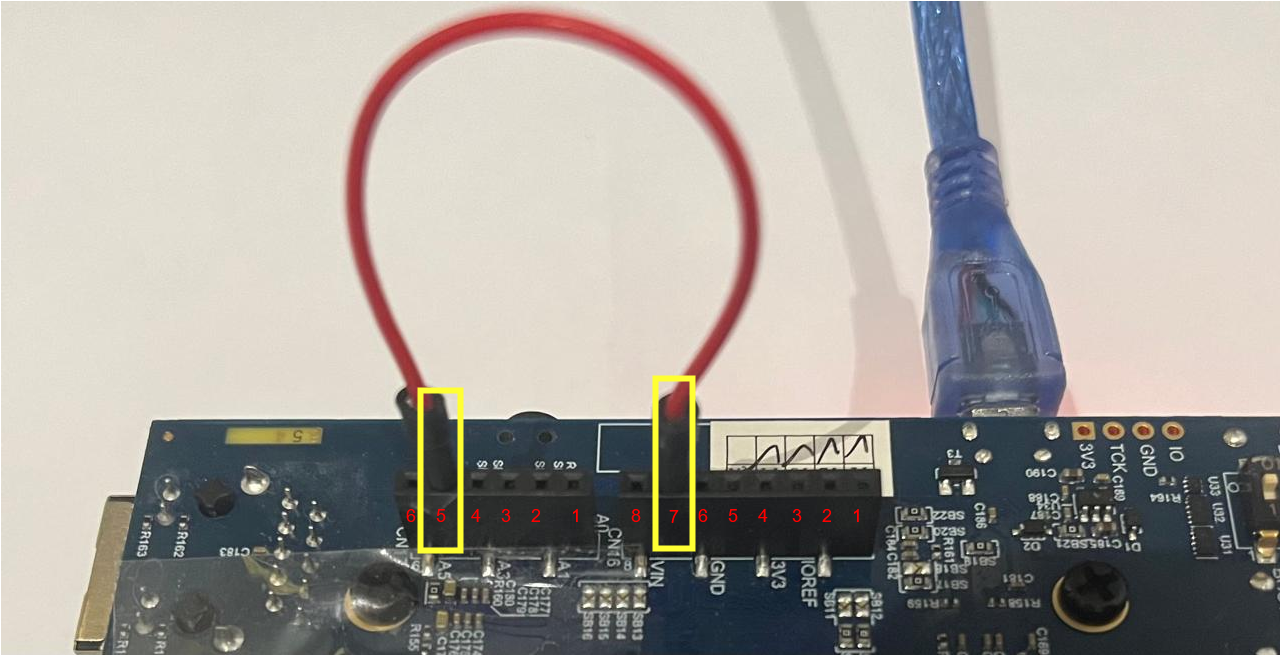
\includegraphics[width=0.68\textwidth]{latex_assets/page8_img1.png}
    \caption{Figura 3 do roteiro oficial: Jumper ligando diretamente o Pino 5 do conector ADC (6 furos à esquerda) ao Pino 6 de \texttt{GND} do conector de alimentação (8 furos à direita) para forçar leitura zero.}
\end{figure}

\begin{labbox}{Roteiro Prático no Laboratório (10 minutos)}
\begin{enumerate}[leftmargin=*]
    \item \textbf{Aterrar o pino do ADC (Conforme Figura 3 acima):} \\
    Com a placa desligada, retire temporariamente o fio de sinal do sensor do \textbf{Pino 5 do conector de 6 furos} e use um cabo jumper Macho-Macho para ligar esse \textbf{Pino 5 (ADC)} diretamente ao \textbf{Pino 6 ou 7 (\texttt{GND})} do bloco de 8 furos ao lado. Isso garante fisicamente que a tensão naquele pino seja exatamente \textbf{0 V}.
    
    \item \textbf{Ligar a Placa e Abrir o Terminal Serial:}
    \begin{itemize}
        \item Conecte o cabo \textbf{USB-C} na porta \texttt{PWR\_IN} (ao lado do conector Ethernet) para alimentar a placa.
        \item Conecte o cabo \textbf{Micro-USB} na porta serial da placa (\texttt{ST-LINK}) e no computador do laboratório.
        \item Abra o programa \textbf{TeraTerm} (no Windows) ou \textbf{minicom} (no Linux), selecione a conexão \textbf{Serial} e configure: \textbf{Baudrate = 115200}, \textbf{8N1} (8 bits, sem paridade, 1 stop bit).
        \item Aperte \texttt{Enter}. Quando pedir login, digite usuário \textbf{\texttt{root}} e senha \textbf{\texttt{root}}.
    \end{itemize}
    
    \item \textbf{Inspecionar os Canais IIO no Terminal da Placa:} \\
    Digite os comandos abaixo no terminal da STM32MP157D-DK1:
\begin{lstlisting}[language=bash]
# Entra na pasta do conversor A/D (subsistema IIO)
cd /sys/bus/iio/devices/iio:device0/

# Lista todos os arquivos disponiveis na pasta
ls

# Mostra o nome de cada canal junto com o valor lido nele
head in_voltage*_raw
\end{lstlisting}
    \item \textbf{Anote o resultado:} O arquivo \texttt{in\_voltageX\_raw} que exibir o valor \textbf{\texttt{0}} (ou muito próximo de zero, ex.: \texttt{1} ou \texttt{2}) enquanto os outros exibem números altos é o seu canal!
    \item \textbf{Teste rápido com o Sensor HW-201 conectado:} Desligue a placa, reconecte os 3 fios do sensor HW-201 (igual à Entrega 0), ligue a placa novamente e rode \texttt{cat in\_voltageX\_raw} duas vezes:
    \begin{itemize}
        \item \textbf{Sem nada na frente do sensor:} Anote o valor alto lido (ex.: \texttt{4095} ou \texttt{65535}).
        \item \textbf{Com a mão ou tampa a 5 cm do sensor:} Veja o LED do sensor acender e anote o valor baixo lido (próximo de \texttt{0}). A média entre esses dois números será o seu \textbf{limiar (\texttt{threshold})} perfeito!
    \end{itemize}
\end{enumerate}
\end{labbox}

% ====================================================================
\section{Passo 2 (Em Casa): Como Simular a Placa no seu PC}
% ====================================================================

Você não precisa estar no laboratório para programar e testar sua classe C++. Como o programa apenas lê um arquivo de texto contendo um número inteiro, você pode criar um ``sensor falso'' (\textit{mock}) no seu computador!

\begin{homebox}{Criando seu Simulador Local em 30 Segundos}
No terminal do seu Linux (ou WSL / Git Bash em casa), crie um arquivo de texto para fingir que é o canal IIO da placa:
\begin{lstlisting}[language=bash]
# Cria uma pasta temporaria para simular o diretorio da placa
mkdir -p /tmp/mock_iio

# Escreve um valor alto (simulando 3,3V -> Sem obstaculo / Tampa aberta)
echo "4095" > /tmp/mock_iio/in_voltage0_raw

# Quando quiser simular um obstaculo/tampa fechada (0V), basta rodar:
echo "120" > /tmp/mock_iio/in_voltage0_raw
\end{lstlisting}
\textbf{Dica de Arquitetura:} Se você programar o construtor da sua classe C++ para receber o \textbf{caminho do arquivo como parâmetro} (deixando o caminho real \texttt{"/sys/bus/iio/devices/iio:device0/in\_voltageX\_raw"} como valor padrão), o seu código funcionará em casa e na placa sem precisar mudar uma única linha!
\end{homebox}

% ====================================================================
\section{Passo 3 (Em Casa): Construindo sua Classe C++ do Zero}
% ====================================================================

Para você aprender de verdade a matéria de Programação Orientada a Objetos (POO), vamos construir a sua classe etapa por etapa. Você mesmo vai criar dois arquivos:
\begin{enumerate}
    \item \texttt{include/IrObstacleSensor.hpp} (O Cabeçalho / Contrato da Classe)
    \item \texttt{src/IrObstacleSensor.cpp} (A Implementação / Lógica dos Métodos)
\end{enumerate}

\subsection{Projetando o Cabeçalho (\texttt{include/IrObstacleSensor.hpp})}

Abra o arquivo \texttt{include/IrObstacleSensor.hpp} em branco e siga estes 4 blocos conceituais:

\begin{theorybox}{Conceito 1: Include Guards (Proteção contra Inclusão Dupla)}
Todo arquivo \texttt{.hpp} deve começar com \texttt{\#ifndef NOME\_HPP}, \texttt{\#define NOME\_HPP} e terminar com \texttt{\#endif}. Isso impede que o compilador dê erro de ``classe redefinida'' caso dois arquivos \texttt{.cpp} façam \texttt{\#include "IrObstacleSensor.hpp"} no futuro.
\end{theorybox}

\textbf{O que você deve declarar dentro da sua \texttt{class IrObstacleSensor}:}
\begin{itemize}[leftmargin=*]
    \item \textbf{Na seção \texttt{private:} (Encapsulamento --- ninguém de fora mexe diretamente):}
    \begin{enumerate}
        \item Uma variável \texttt{std::string} (ex.: \texttt{devicePath}) para guardar o caminho do arquivo IIO.
        \item Uma variável \texttt{int} (ex.: \texttt{lastRawValue}) para guardar o último número lido do ADC.
        \item Uma variável \texttt{int} (ex.: \texttt{threshold}) para guardar o limiar que separa nível BAIXO (0 V) de nível ALTO (3,3 V).
    \end{enumerate}
    
    \item \textbf{Na seção \texttt{public:} (A interface que o resto do programa pode chamar):}
    \begin{enumerate}
        \item \textbf{O Construtor:} Tem o mesmo nome da classe e não tem tipo de retorno. Use argumentos padrão (\textit{default arguments}) para facilitar o uso:
        \begin{lstlisting}[language=C++]
explicit IrObstacleSensor(
    const std::string& path = "/sys/bus/iio/devices/iio:device0/in_voltage0_raw",
    int alertThreshold = 2000
);
        \end{lstlisting}
        \item \textbf{Método de Leitura Bruta (\texttt{int readRaw();}):} Abre o arquivo, atualiza \texttt{lastRawValue} e retorna o inteiro lido.
        \item \textbf{Método de Interpretação Física (\texttt{bool isObstacleDetected() const;}):} Lembra que o sensor HW-201 é \textit{Active-Low}? Quando há obstáculo/reflexão, a tensão cai para 0 V (\texttt{lastRawValue < threshold}).
        \item \textbf{Getters e Setters:} Ex.: \texttt{int getLastRawValue() const;} e \texttt{void setThreshold(int newThreshold);}. \\
        \textit{Pergunta de prova:} Por que colocamos a palavra \texttt{const} no final de \texttt{getLastRawValue() const}? Porque isso promete ao compilador que esse método apenas lê dados e \textbf{não modifica} nenhum atributo da classe!
    \end{enumerate}
\end{itemize}

\subsection{Programando a Lógica (\texttt{src/IrObstacleSensor.cpp})}

No arquivo \texttt{src/IrObstacleSensor.cpp}, você começa com \texttt{\#include "IrObstacleSensor.hpp"}, \texttt{\#include <fstream>} (para ler arquivos) e \texttt{\#include <stdexcept>} (para lançar erros caso o arquivo não exista).

\begin{theorybox}{Conceito 2: Como implementar os métodos usando o operador de escopo \texttt{::}}
Fora do \texttt{.hpp}, para avisar ao compilador que uma função pertence à sua classe, você escreve \texttt{NomeDaClasse::nomeDoMetodo(...)}. Veja como funciona a leitura de arquivo em C++ com \texttt{std::ifstream}:
\begin{lstlisting}[language=C++]
int IrObstacleSensor::readRaw() {
    // 1. Cria um objeto ifstream tentando abrir o arquivo no caminho devicePath
    std::ifstream file(devicePath);

    // 2. Verifica se o arquivo abriu com sucesso
    if (!file.is_open()) {
        throw std::runtime_error("Erro ao abrir o canal IIO: " + devicePath);
    }

    // 3. Usa o operador de extracao (>>) para ler o inteiro do arquivo para o atributo
    file >> lastRawValue;

    // 4. Retorna o valor lido (o arquivo se fecha sozinho ao sair da funcao!)
    return lastRawValue;
}
\end{lstlisting}
\textit{Por que não precisamos dar \texttt{file.close()}?} Porque em C++ moderno o destrutor de \texttt{std::ifstream} fecha o arquivo automaticamente assim que a função termina (princípio chamado \textbf{RAII}).
\end{theorybox}

% ====================================================================
\section{Passo 4 (Em Casa): Documentando com Doxygen}
% ====================================================================

O edital exige que sua classe esteja documentada com \textbf{Doxygen}. O Doxygen é um programa que lê comentários especiais no formato \texttt{/** ... */} dentro do seu código e gera um site HTML completo de documentação.

\begin{homebox}{Como Escrever Comentários Doxygen no seu \texttt{.hpp}}
Coloque blocos \texttt{/** ... */} imediatamente acima da classe e de cada método no seu \texttt{IrObstacleSensor.hpp}, usando as tags principais:
\begin{itemize}[leftmargin=*]
    \item \texttt{@file}: Nome do arquivo e resumo do propósito dele (no topo do arquivo).
    \item \texttt{@class}: Nome da classe e explicação geral.
    \item \texttt{@brief}: Uma frase curta explicando o que o método ou atributo faz.
    \item \texttt{@param nome}: Explica para que serve cada parâmetro que o método recebe.
    \item \texttt{@return}: Explica o que o método devolve quando termina.
\end{itemize}

\textbf{Exemplo de como documentar um método:}
\begin{lstlisting}[language=C++]
/**
 * @brief Avalia se o feixe infravermelho detectou um obstaculo ou reflexao.
 * @details No modulo HW-201 (LM393), a deteccao de reflexao leva a saida para 0V.
 * @return true se a leitura estiver abaixo do limiar (obstaculo presente), false caso contrario.
 */
bool isObstacleDetected() const;
\end{lstlisting}

\textbf{Como testar a geração do Doxygen no terminal:}
\begin{lstlisting}[language=bash]
# 1. Gera um arquivo de configuracao padrao chamado Doxyfile
doxygen -g Doxyfile

# 2. (Dica) Abra o Doxyfile num editor de texto e mude a linha INPUT para:
#    INPUT = include src
#    E mude EXTRACT_PRIVATE = YES para documentar tambem seus atributos privados!

# 3. Rode o Doxygen para gerar a pasta html/
doxygen Doxyfile
\end{lstlisting}
Depois, abra o arquivo \texttt{html/index.html} no seu navegador e veja se todos os seus métodos aparecem documentados!
\end{homebox}

% ====================================================================
\section{Passo 5: Compilando, Testando e Entregando (Até 26/10)}
% ====================================================================

Para testar se a sua classe não tem nenhum erro de compilação antes de subir para o GitHub, crie um arquivo simples \texttt{src/main.cpp} que instancia um objeto \texttt{IrObstacleSensor} apontando para o seu arquivo simulado e imprime o resultado no terminal:

\begin{lstlisting}[language=bash]
# Compila o seu codigo com todos os avisos ligados (-Wall -Wextra)
g++ -Wall -Wextra -std=c++17 -Iinclude src/IrObstacleSensor.cpp src/main.cpp -o teste_sensor

# Executa o seu programa
./teste_sensor
\end{lstlisting}

\subsection{Checklist Final para o Commit da Entrega 1}
\begin{enumerate}[leftmargin=*]
    \item[$\square$] Verifique se \textbf{não existe nenhuma variável global} nem função solta fora da classe nos seus arquivos \texttt{.hpp} e \texttt{.cpp}.
    \item[$\square$] Atualize o \texttt{README.md} explicando a estrutura da sua classe \texttt{IrObstacleSensor}, seus atributos privados, seus métodos públicos e como compilar/gerar a documentação Doxygen.
    \item[$\square$] Faça o commit e suba para o GitHub:
    \begin{lstlisting}[language=bash]
git add include/ src/ Doxyfile README.md
git commit -m "Entrega 1: Implementacao da classe IrObstacleSensor com Doxygen"
git push origin main
    \end{lstlisting}
    \item[$\square$] \textbf{Como pegar o Link do Commit Final exigido no Google Classroom:} \\
    Entre na página do seu repositório no GitHub, clique em \textbf{``Commits''} (no canto superior direito da lista de arquivos), clique sobre o título do último commit que você acabou de enviar e \textbf{copie a URL completa do navegador} (formato \texttt{https://github.com/usuario/repo/commit/a1b2c3d4...}). Cole esse link na tarefa \textbf{[Projeto] Entrega 1} do Google Classroom!
\end{enumerate}

\subsection{Links Oficiais do Edital (Já Adiante para a Entrega 2 --- 02/11)}
Extraídos diretamente do PDF atualizado do professor (\texttt{Projeto\_de\_Programacao\_Aplicada\_2026 (1).pdf}):
\begin{itemize}[leftmargin=*]
    \item \textbf{Download da Toolchain ARM (\texttt{arm-buildroot-linux-gnueabihf\_sdk-DK2.tar.gz}):} \\
    \url{https://drive.google.com/drive/folders/1wr7YHFre0kxdnQLaE4kMThYUD1u1lBhI?usp=sharing}
    \item \textbf{Tutorial Oficial de Criação da Máquina Virtual Ubuntu no VirtualBox:} \\
    \url{https://ubuntu.com/tutorials/how-to-run-ubuntu-desktop-on-a-virtual-machine-using-virtualbox}
\end{itemize}

\end{document}
